\section{Analysis Metric 2: Package Size}
\label{sec:analysisPackageSize}

The second metric is the uncompressed size of an \ac{NPM} package version, expressed in bytes.
It is relevant because all four \acp{SSCA} introduce or modify files that increase the package size.
Attack~A (\cref{sec:attackA}) adds a \ac{DLL} of 1.2~MB,
Attack~B (\cref{sec:attackB}) increases an existing JavaScript file by adding a malicious line of 76,438 characters,
Attack~C (\cref{sec:attackC}) adds a malicious file weighing approximately 3.7~MB,
and Attack~D (\cref{sec:attackD}) introduces a malicious file weighing over 10~MB.
The question is whether these size increases are large enough to be distinguishable from size changes that occur naturally during benign development.

\subsection{Analysis of the Goodware Dataset}
\label{subsec:goodwarePackageSize}

\begin{figure}[htbp]
    \centering
    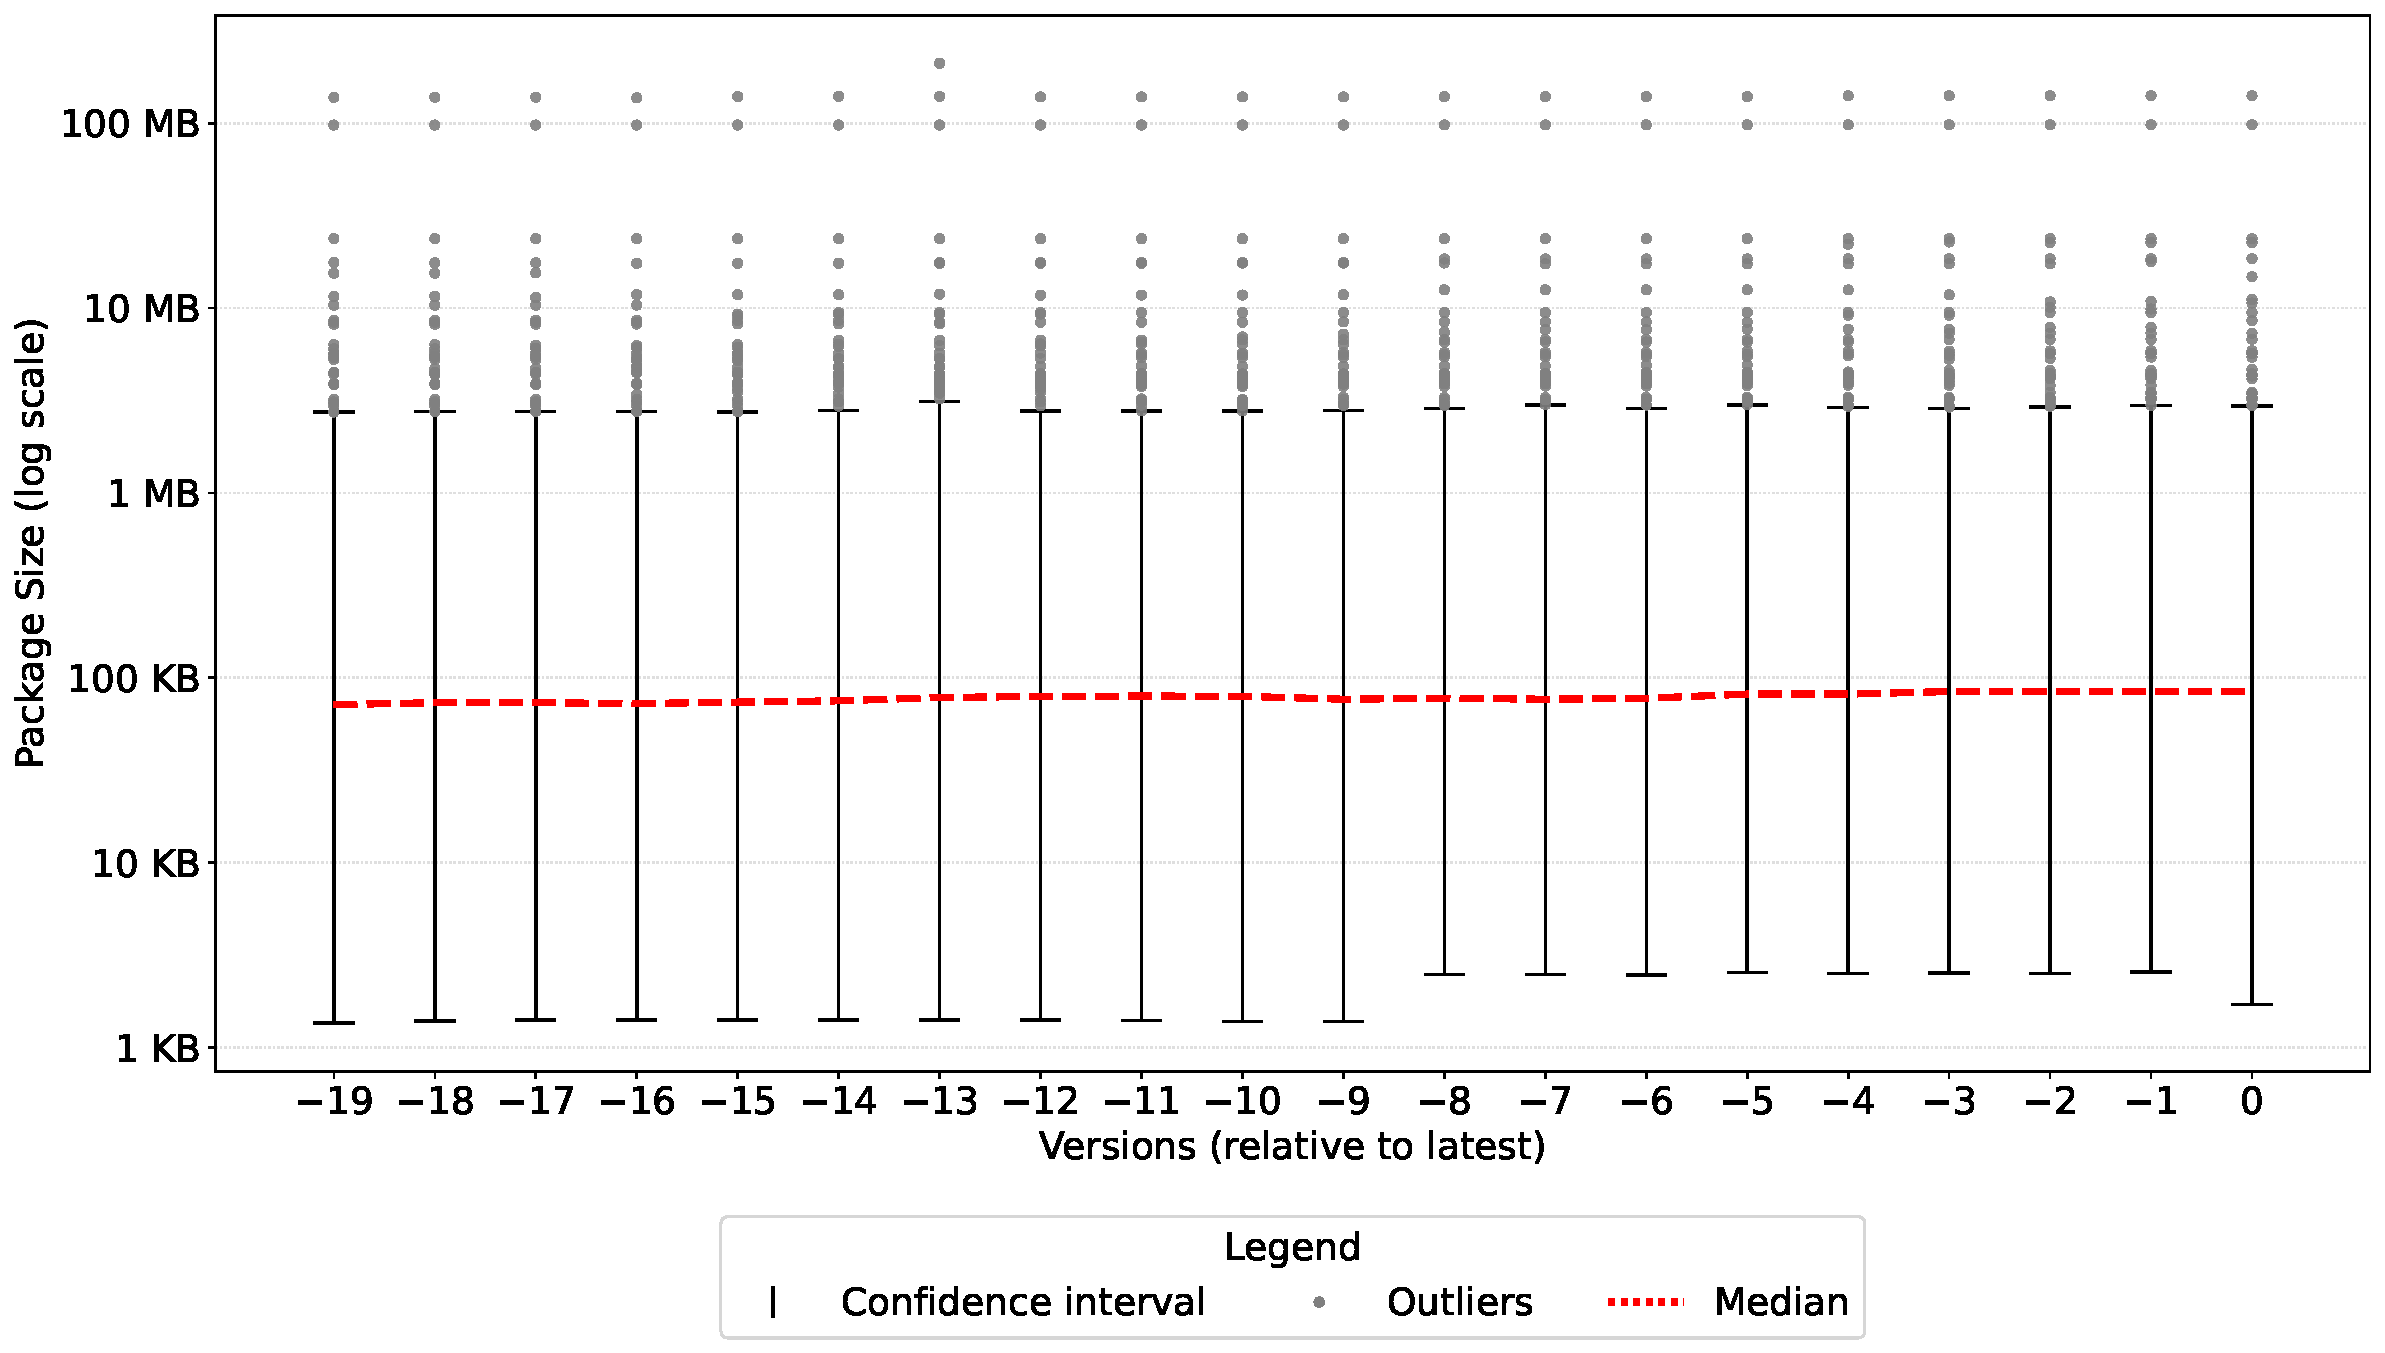
\includegraphics[width=\textwidth]{metrics/packageSize/PS_plot1.pdf}
    \caption{Package Size Metric: Package Trend in Goodware Dataset.}
    \label{fig:fig1PackageSize}
\end{figure}

The Goodware dataset provides, for each of the 629 packages,
the total size observed in each of their 20 analyzed versions, as described in \cref{subsec:goodwareDataset}.
To visualize the distribution and evolutionary patterns of this metric across releases,
we used \cref{fig:fig1PackageSize,fig:fig1PackageSizeIncreasing,fig:fig1PackageSizeDecreasing,fig:fig1PackageSizeStable}.
Among the packages in the Goodware dataset, several exhibit outlier values for one or more versions. 
Nine packages were selected for individual analysis as representative cases, chosen to cover the range of observed trends
and the most common causes of legitimate outlier values, 
such as accidental inclusions, major refactorings, and inherent package characteristics. 
Understanding these patterns is essential to distinguish legitimate anomalies from malicious injections when evaluating the Malware dataset in \cref{subsec:analysisPackageSizeComparisonMalware}.
The following figures highlight these nine packages with solid colored lines, categorizing them according to their observed trends:
\begin{itemize}
    \item \textbf{Increasing Trend} (\cref{fig:fig1PackageSizeIncreasing}): illustrates highlighted packages with an increasing trend over time.
    \item \textbf{Decreasing Trend} (\cref{fig:fig1PackageSizeDecreasing}): shows highlighted packages characterized by a reduction in size.
    \item \textbf{Stable Trend} (\cref{fig:fig1PackageSizeStable}): displays highlighted packages maintaining a constant size throughout their history.
\end{itemize}

\begin{figure}[htbp]
    \centering
    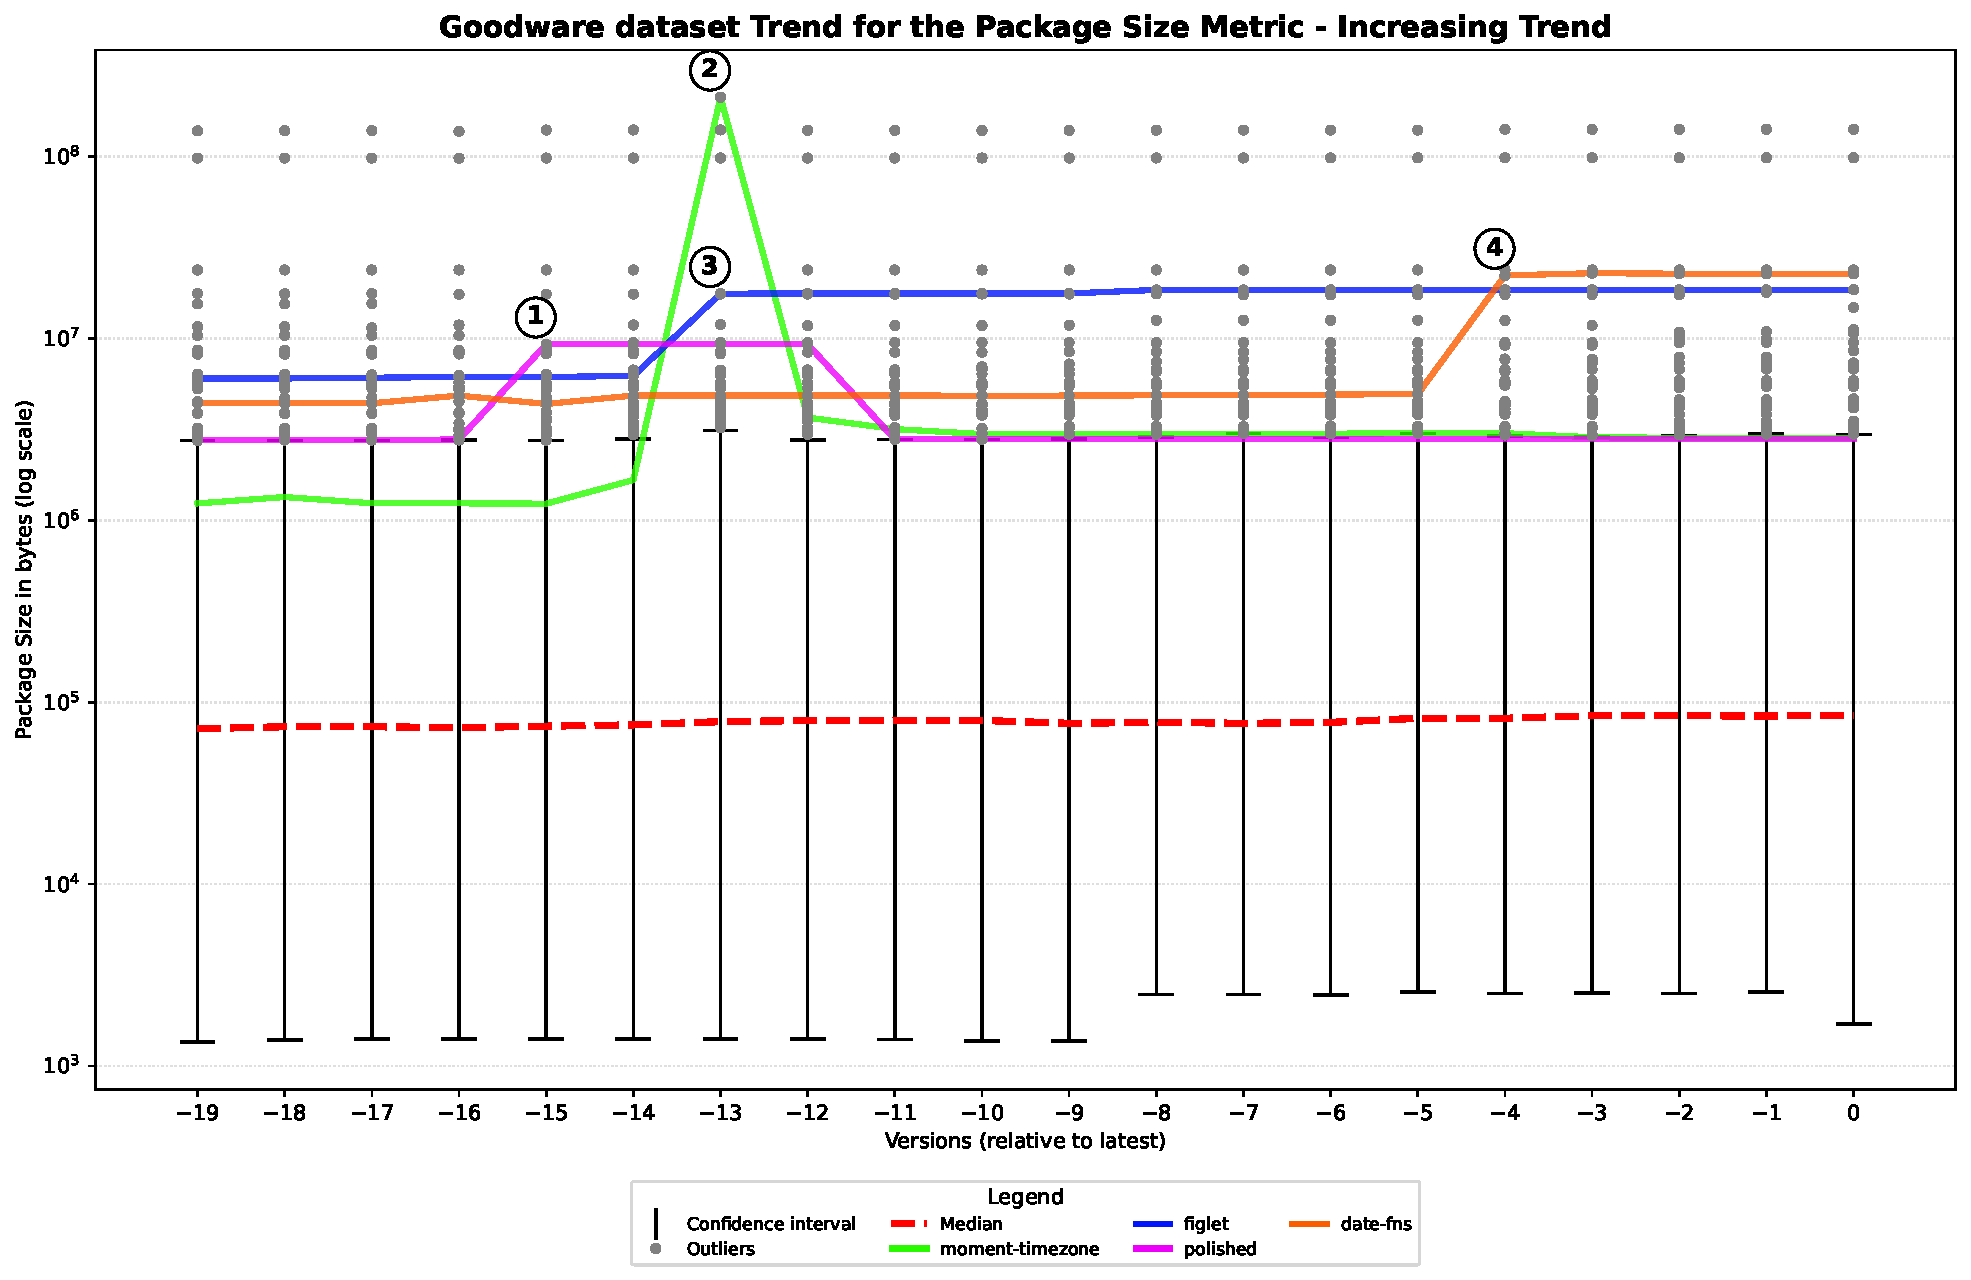
\includegraphics[width=\textwidth]{metrics/packageSize/PS_plot1_Increasing_Trend.pdf}
    \caption{Package Size Metric: Outliers Package Increasing Trend in Goodware Dataset.}
    \label{fig:fig1PackageSizeIncreasing}
\end{figure}

\cref{fig:fig1PackageSizeIncreasing} shows four packages that experienced a significant size increase across versions:
\texttt{polished}, \texttt{moment-timezone}, \texttt{figlet}, and \texttt{date-fns}.

\textbf{polished} (solid pink line) is a package used for styling in JavaScript~\cite{polished}.
As seen at point~1 in \cref{fig:fig1PackageSizeIncreasing}, it grew from about 2.7~MB to 9.2~MB
starting from version 4.0.0-beta.2 for four consecutive releases.
In these versions, the developers erroneously included a \texttt{.yarn} cache directory in the final tarball distributed to the public, 
which contained numerous files, as also discussed in \cref{subsec:analysisFileTypesGoodware}.
The package returned to its previous size in version 4.0.4 once the folder was removed, 
as reported in the release notes on GitHub~\cite{polished_release_notes}.

As seen at point~2 in \cref{fig:fig1PackageSizeIncreasing},
\textbf{moment-timezone} (solid green line) jumped from about 1.6~MB to 211~MB in version 0.5.36
due to the accidental inclusion of a temporary folder, 
making this the heaviest tarball in the entire Goodware dataset.
The folder was removed in the following release.
    
\textbf{figlet} (solid blue line) is used to create ASCII art text from normal strings,
transforming letters into large stylized characters composed of symbols~\cite{figlet}.
As seen at point~3 in \cref{fig:fig1PackageSizeIncreasing},
it grew from about 6.2~MB to 17.5~MB in version 1.9.0, 
when the project underwent a major refactoring to adopt TypeScript and modern build tooling, 
adding approximately 300 new files, as reported in the release notes on GitHub~\cite{figlet_release_notes}.
This is an example of a legitimate, planned size increase with a clear documented cause.

\textbf{date-fns} (solid orange line) provides a toolset for manipulating JavaScript dates in a browser and Node.js~\cite{date-fns}.
As seen at point~4 in \cref{fig:fig1PackageSizeIncreasing},
it grew from about 5~MB to 22~MB in release 3.6.0, when the developers added 400 new files for compatibility with older browsers~\cite{date-fns_release_notes}.
Again, this is a documented and legitimate change.

These examples illustrate as large size increases can occur in benign packages for a variety of reasons, 
such as accidental inclusions, refactoring, or intentional feature additions.

\begin{figure}[htbp]
    \centering
    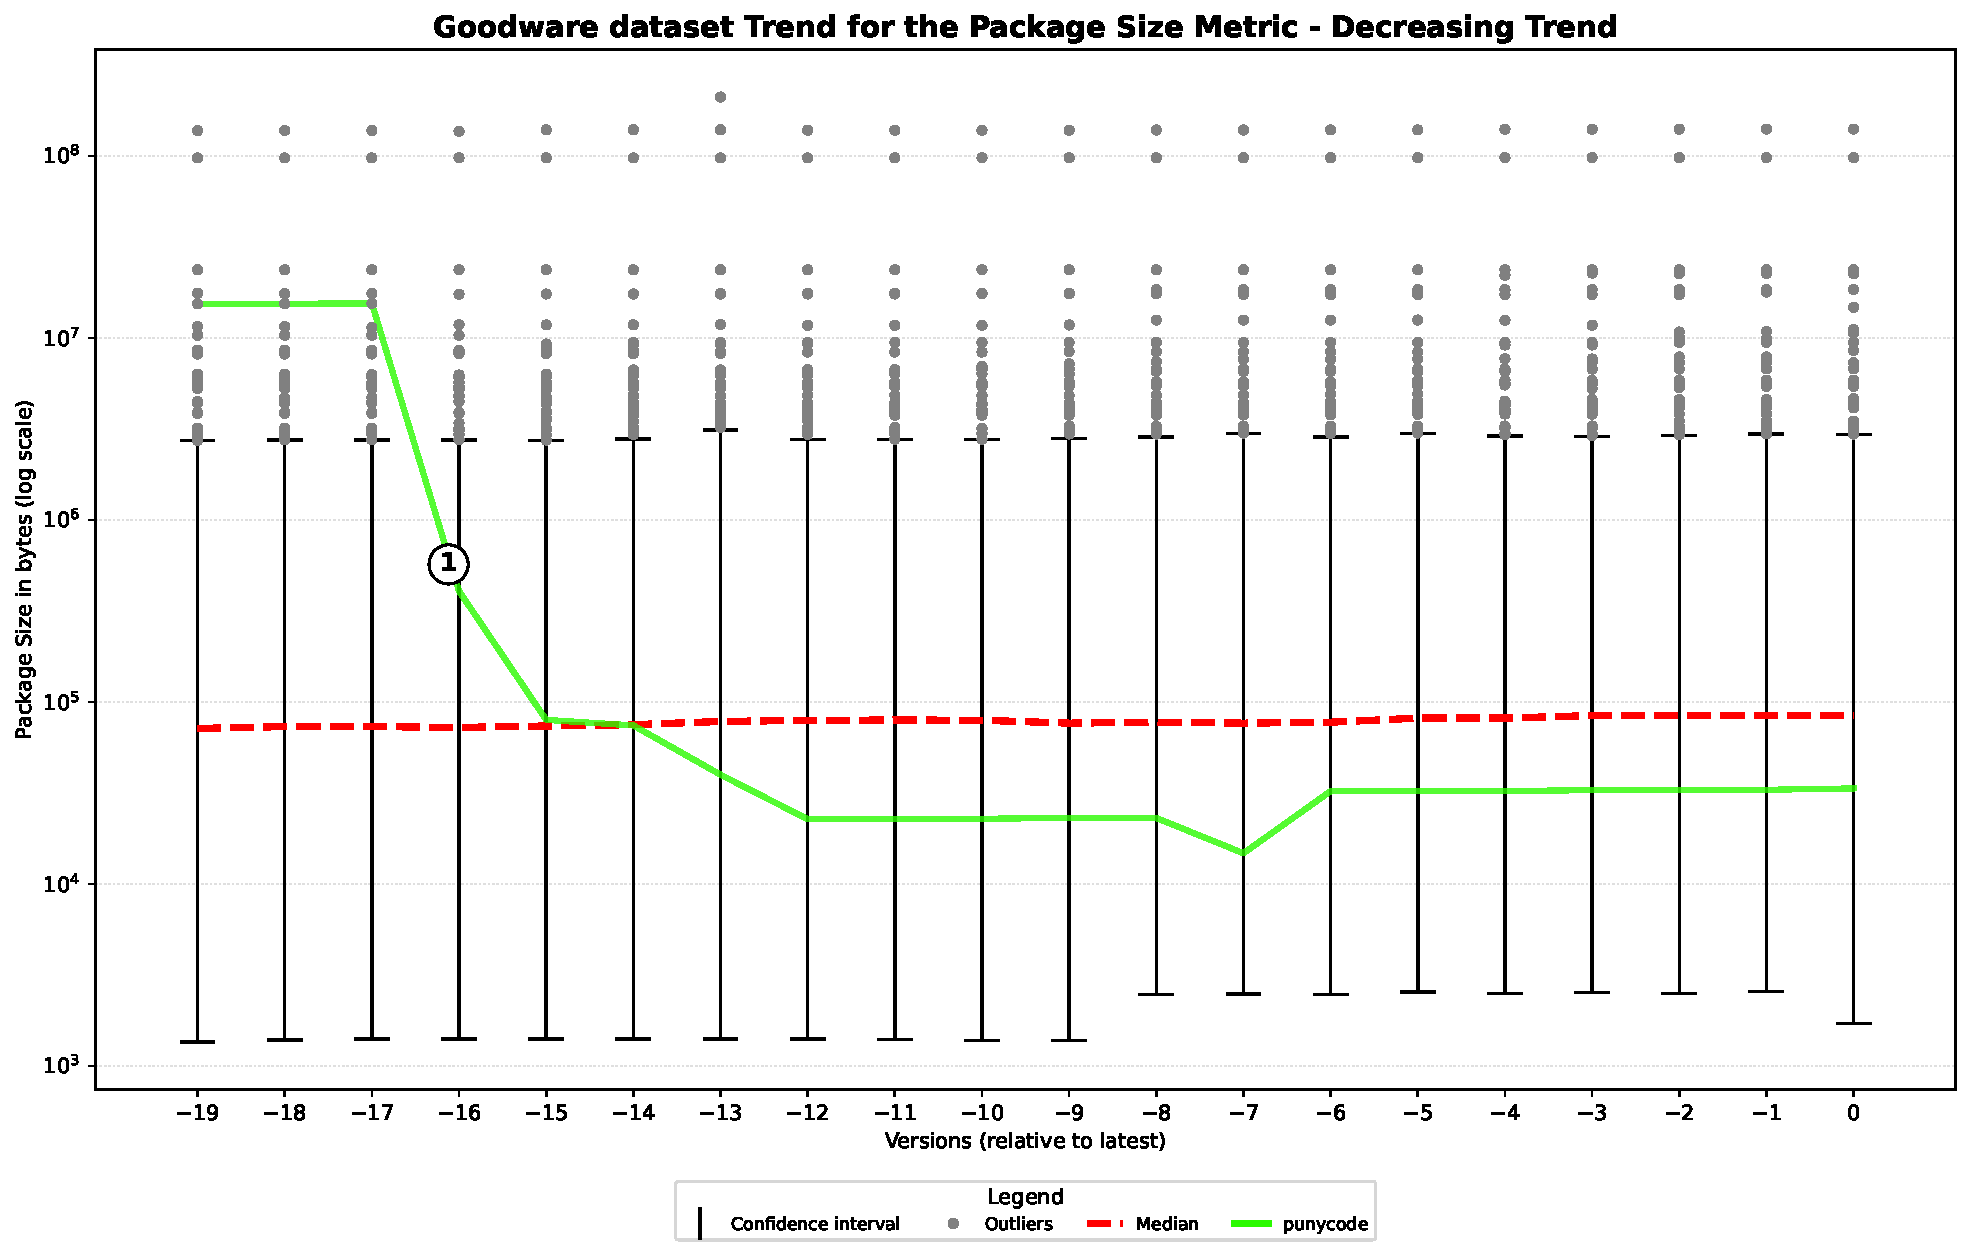
\includegraphics[width=\textwidth]{metrics/packageSize/PS_plot1_Decreasing_Trend.pdf}
    \caption{Package Size Metric: Outliers Package Decreasing Trend in Goodware Dataset.}
    \label{fig:fig1PackageSizeDecreasing}
\end{figure}

Only the \texttt{punycode} package (solid green line in \cref{fig:fig1PackageSizeDecreasing}) 
experienced a decrease enough to move from an outlier to within the confidence interval between consecutive releases.
In the first three versions, it started with a size of 15.5~MB,
and from point~1 in \cref{fig:fig1PackageSizeDecreasing}, 
it was progressively optimized to include only the essential files,
shrinking to approximately 33~KB in its most recent releases.
This represents a deliberate and documented cleanup of the distribuited tarball.

\begin{figure}[htbp]
    \centering
    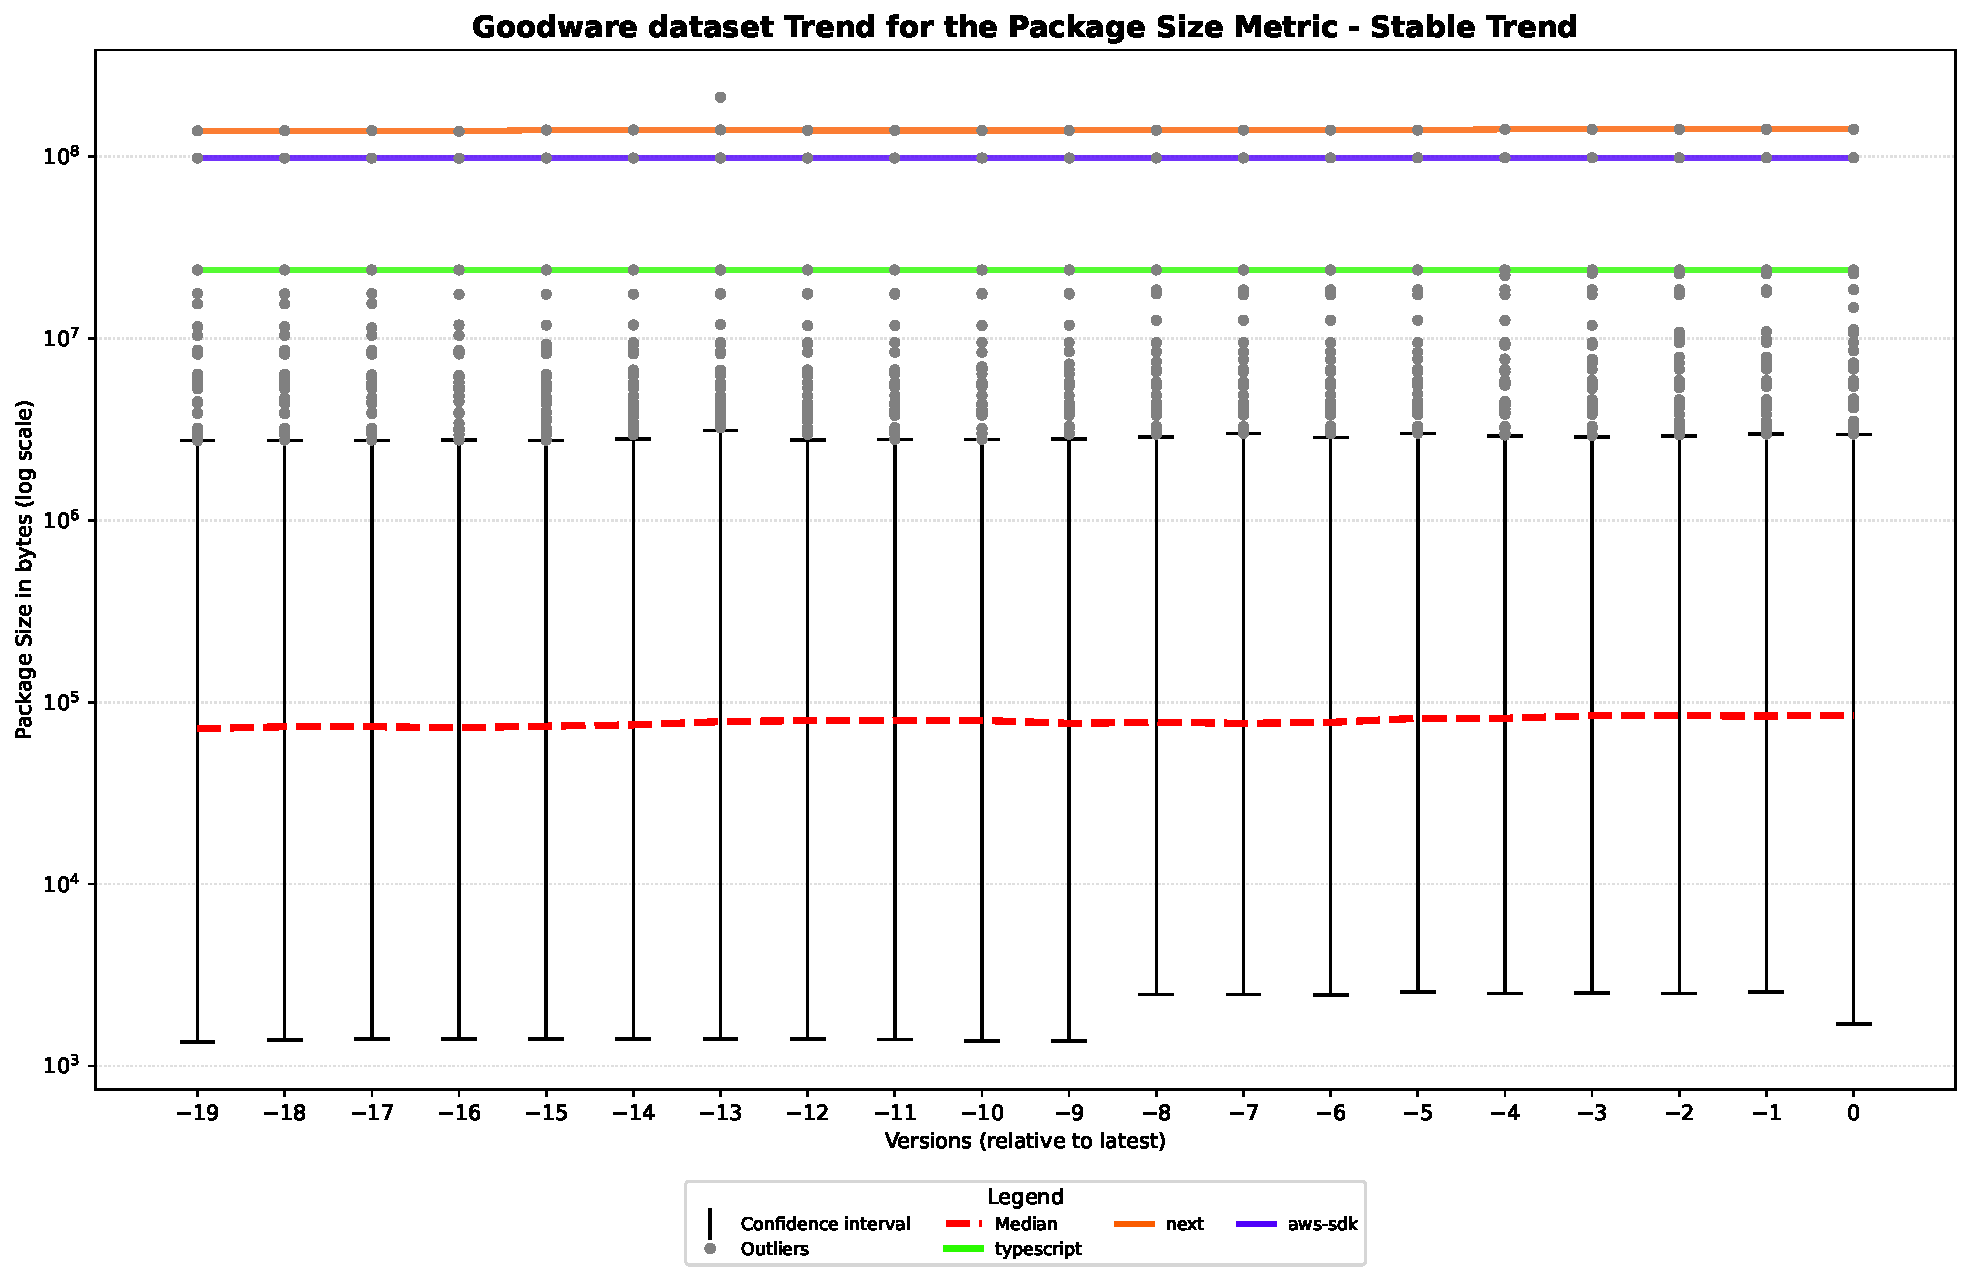
\includegraphics[width=\textwidth]{metrics/packageSize/PS_plot1_Stable_Trend.pdf}
    \caption{Package Size Metric: Outliers Package Stable Trend in Goodware Dataset.}
    \label{fig:fig1PackageSizeStable}
\end{figure}

As shown in \cref{fig:fig1PackageSizeStable},
three packages are consistently the largest in the dataset across all 20 versions:
\texttt{next}~\cite{next} (solid orange, 140~MB, a React full-stack framework),
\texttt{aws-sdk}~\cite{aws-sdk} (solid purple, 98~MB, the official \ac{AWS} client),
and \texttt{typescript}~\cite{typescript} (solid green, 23.7~MB, the TypeScript compiler).

\subsection{Comparison with the Malware Dataset}
\label{subsec:analysisPackageSizeComparisonMalware}

\begin{figure}[htbp]
    \centering
    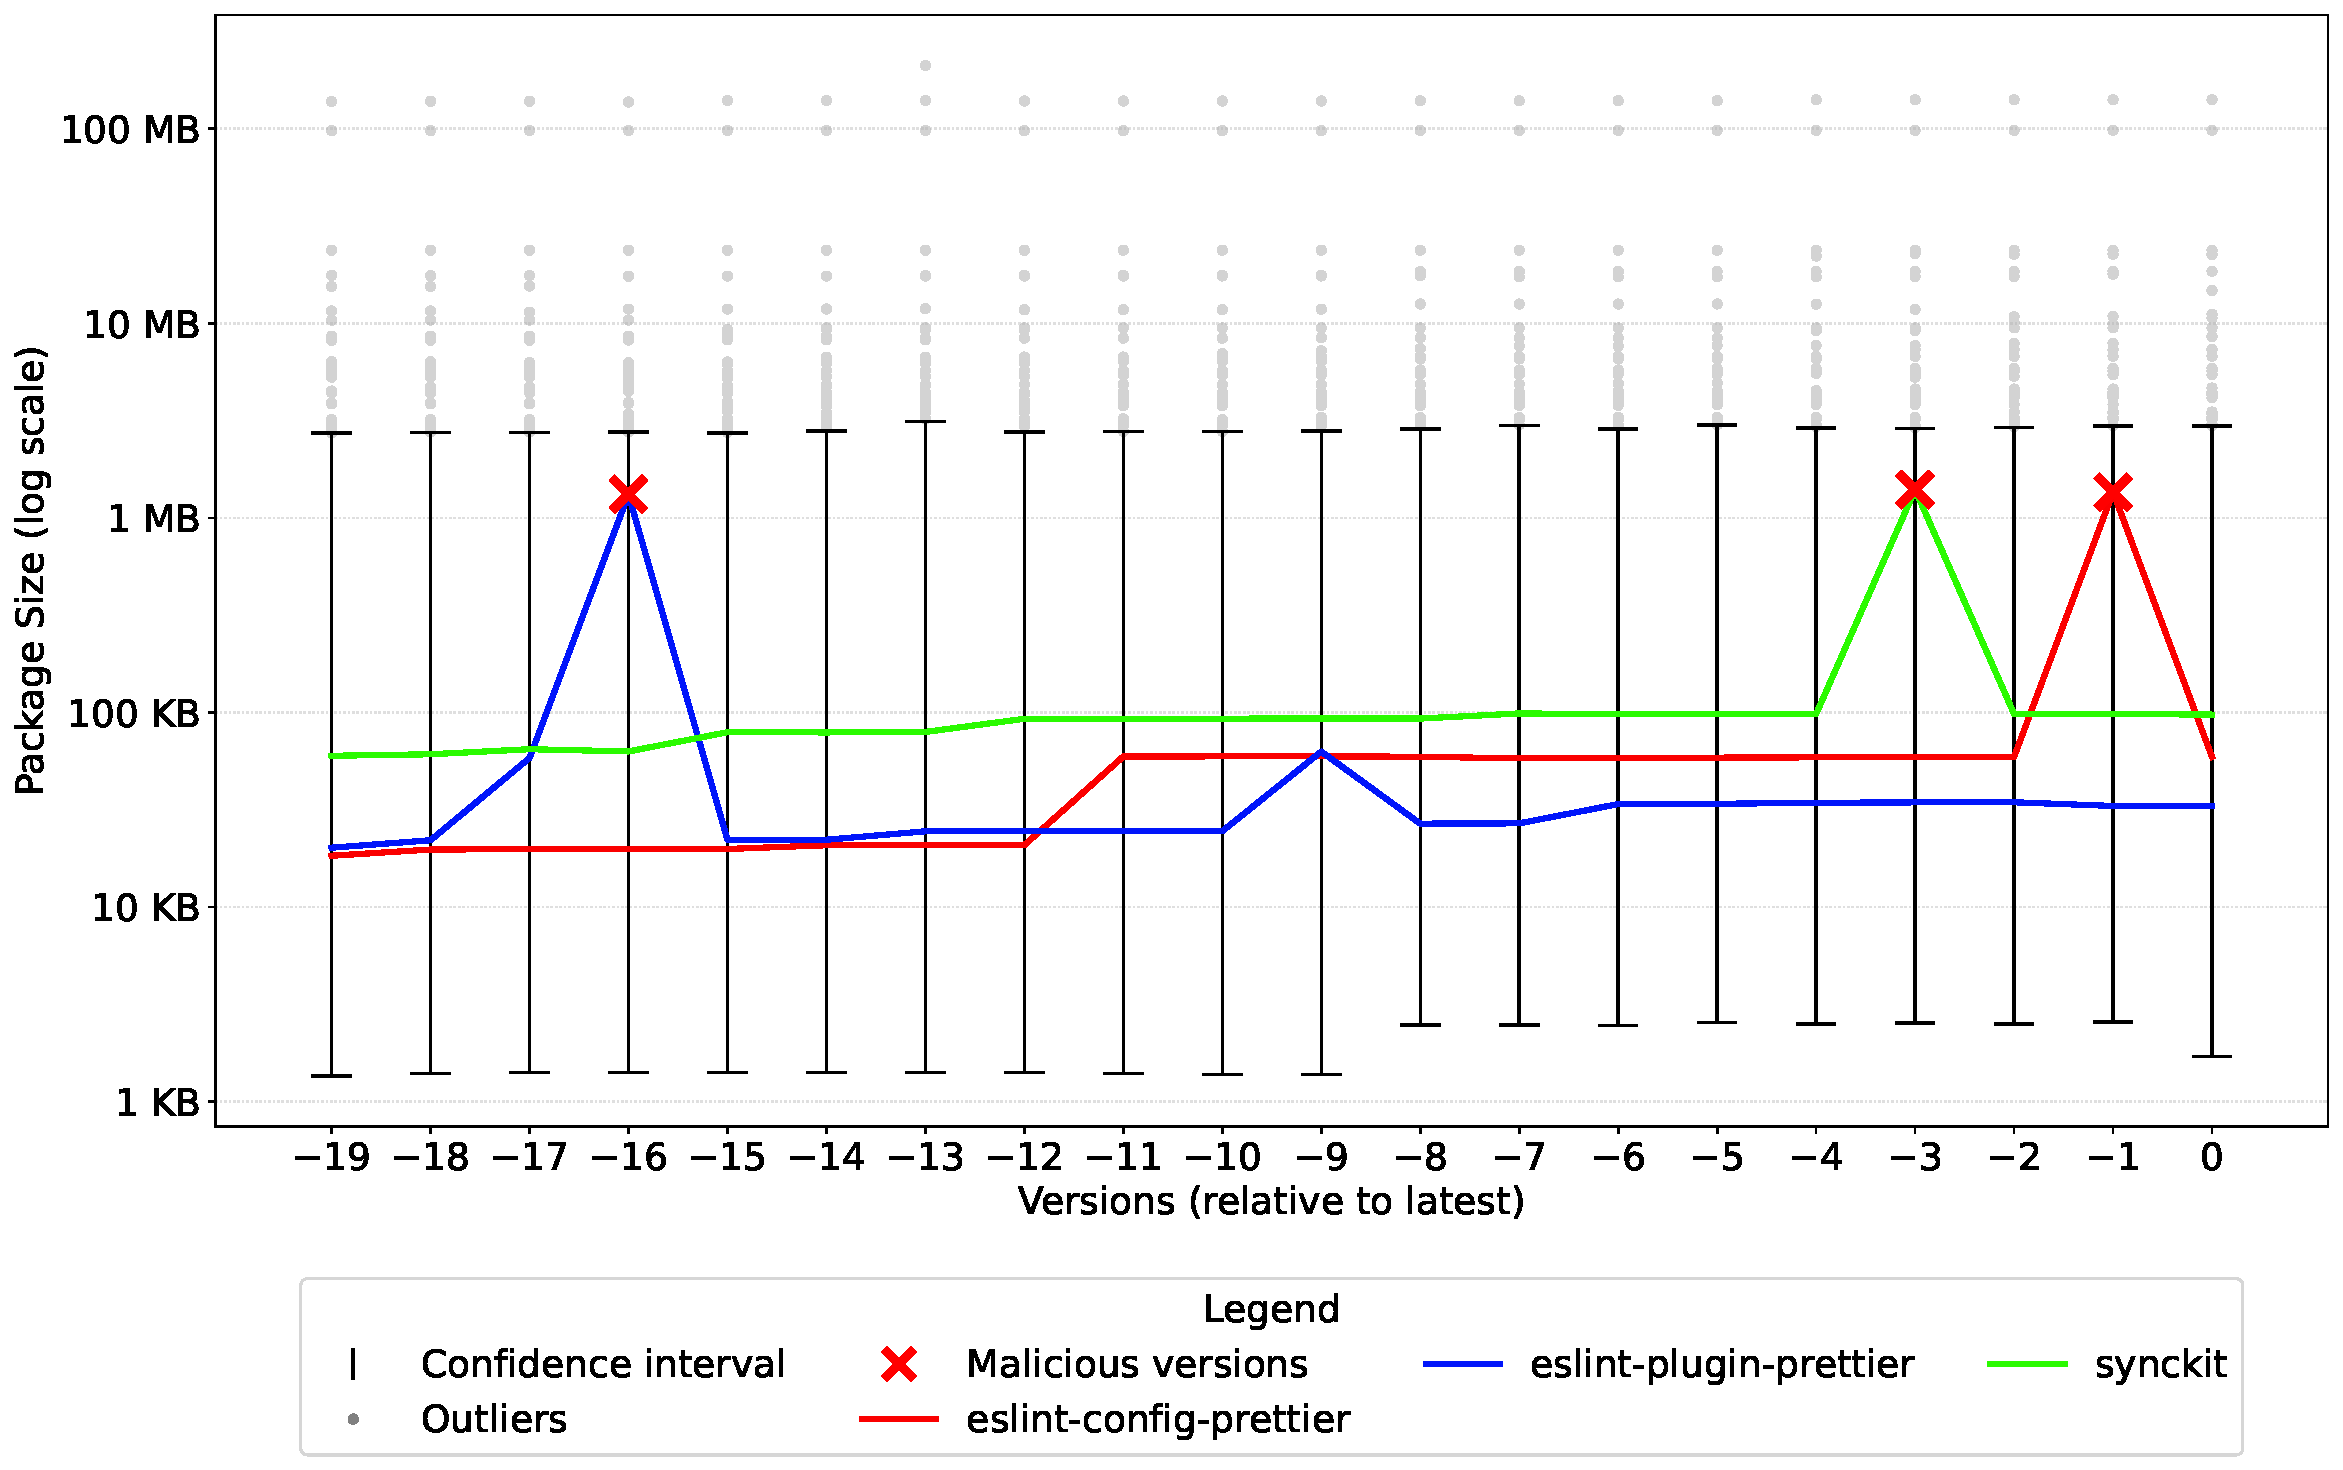
\includegraphics[width=\textwidth]{metrics/packageSize/PS_plot2single_AttackA.pdf}
    \caption{Package Size Metric: Malware Comparison for Attack A.}
    \label{fig:fig2PackageSizeAttackA}
\end{figure}

\begin{figure}[htbp]
    \centering
    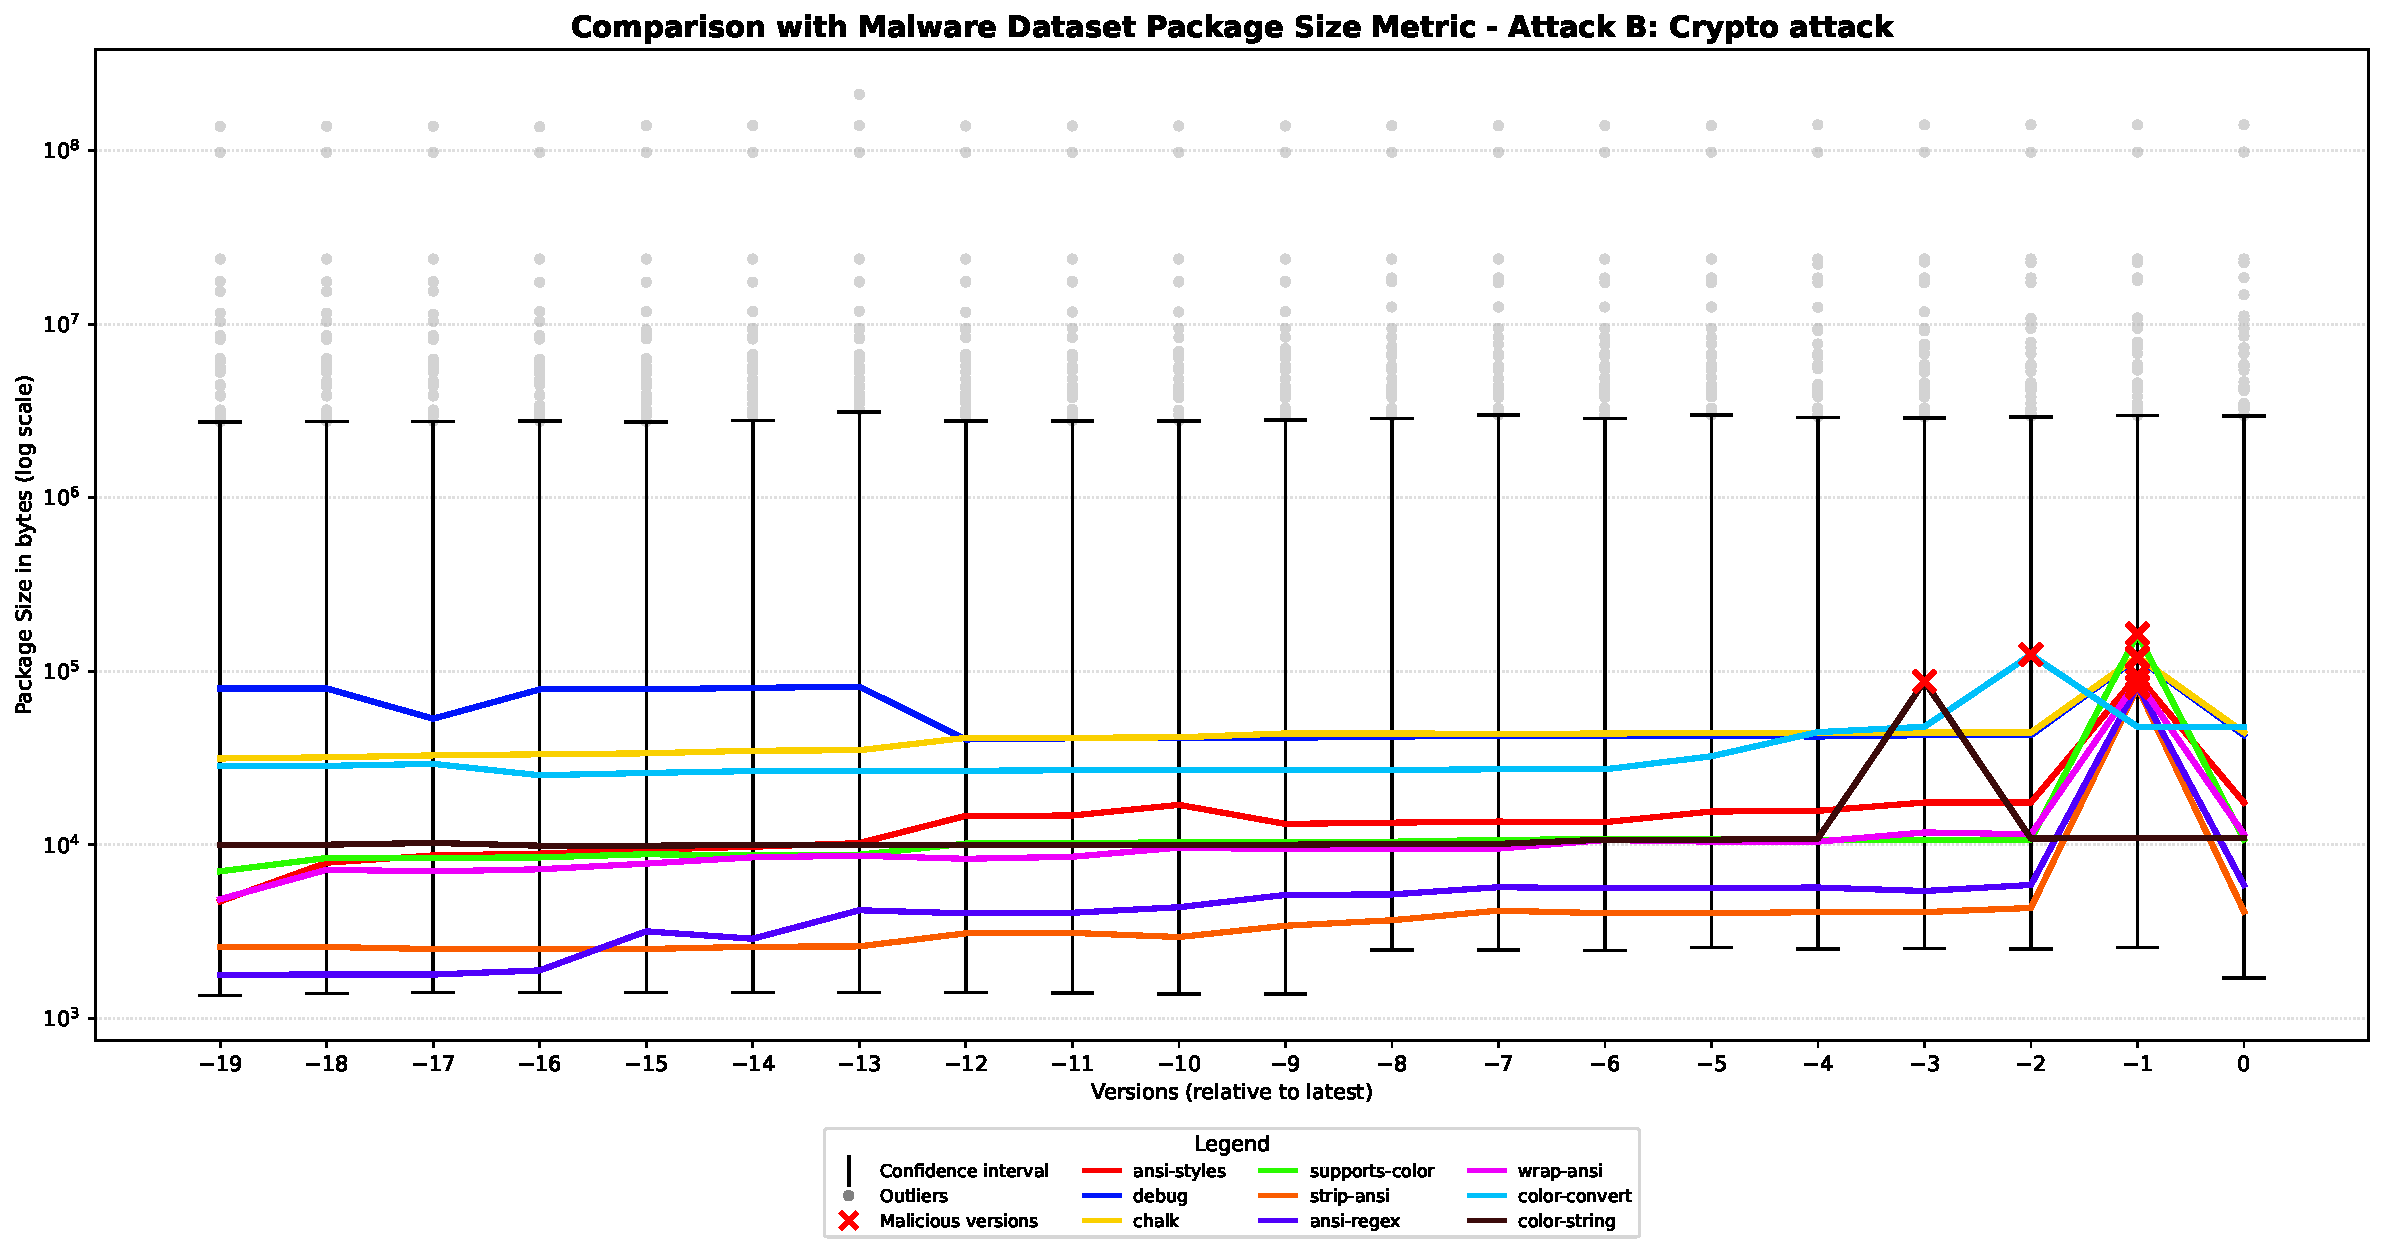
\includegraphics[width=\textwidth]{metrics/packageSize/PS_plot2single_AttackB.pdf}
    \caption{Package Size Metric: Malware Comparison for Attack B.}
    \label{fig:fig2PackageSizeAttackB}
\end{figure}

\begin{figure}[htbp]
    \centering
    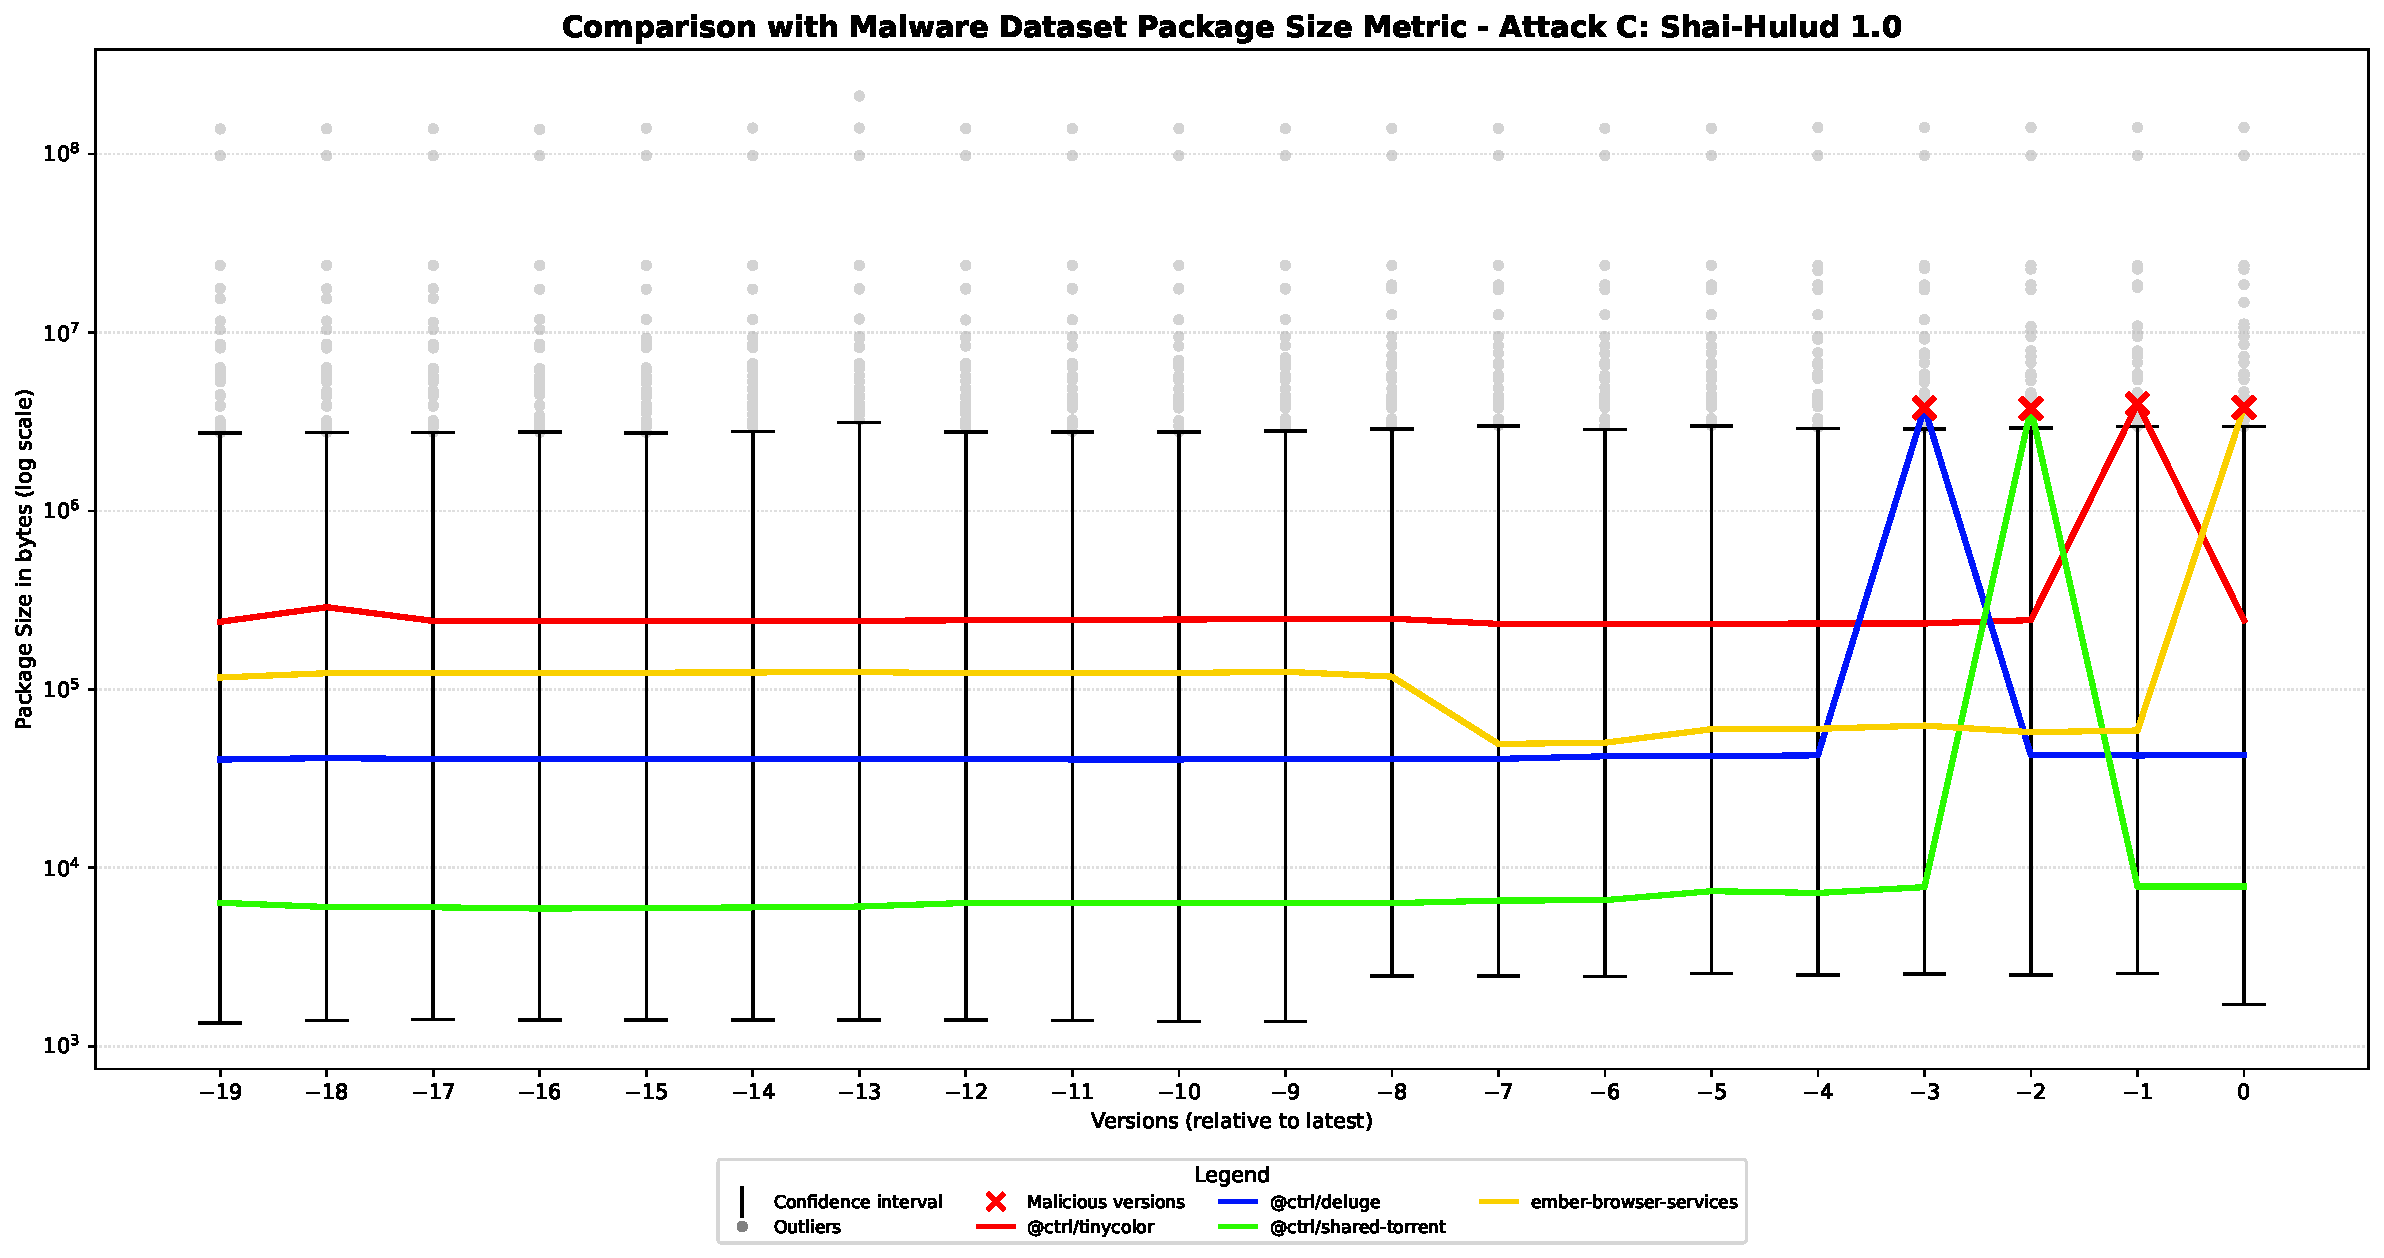
\includegraphics[width=\textwidth]{metrics/packageSize/PS_plot2single_AttackC.pdf}
    \caption{Package Size Metric: Malware Comparison for Attack C.}
    \label{fig:fig2PackageSizeAttackC}
\end{figure}

\begin{figure}[htbp]
    \centering
    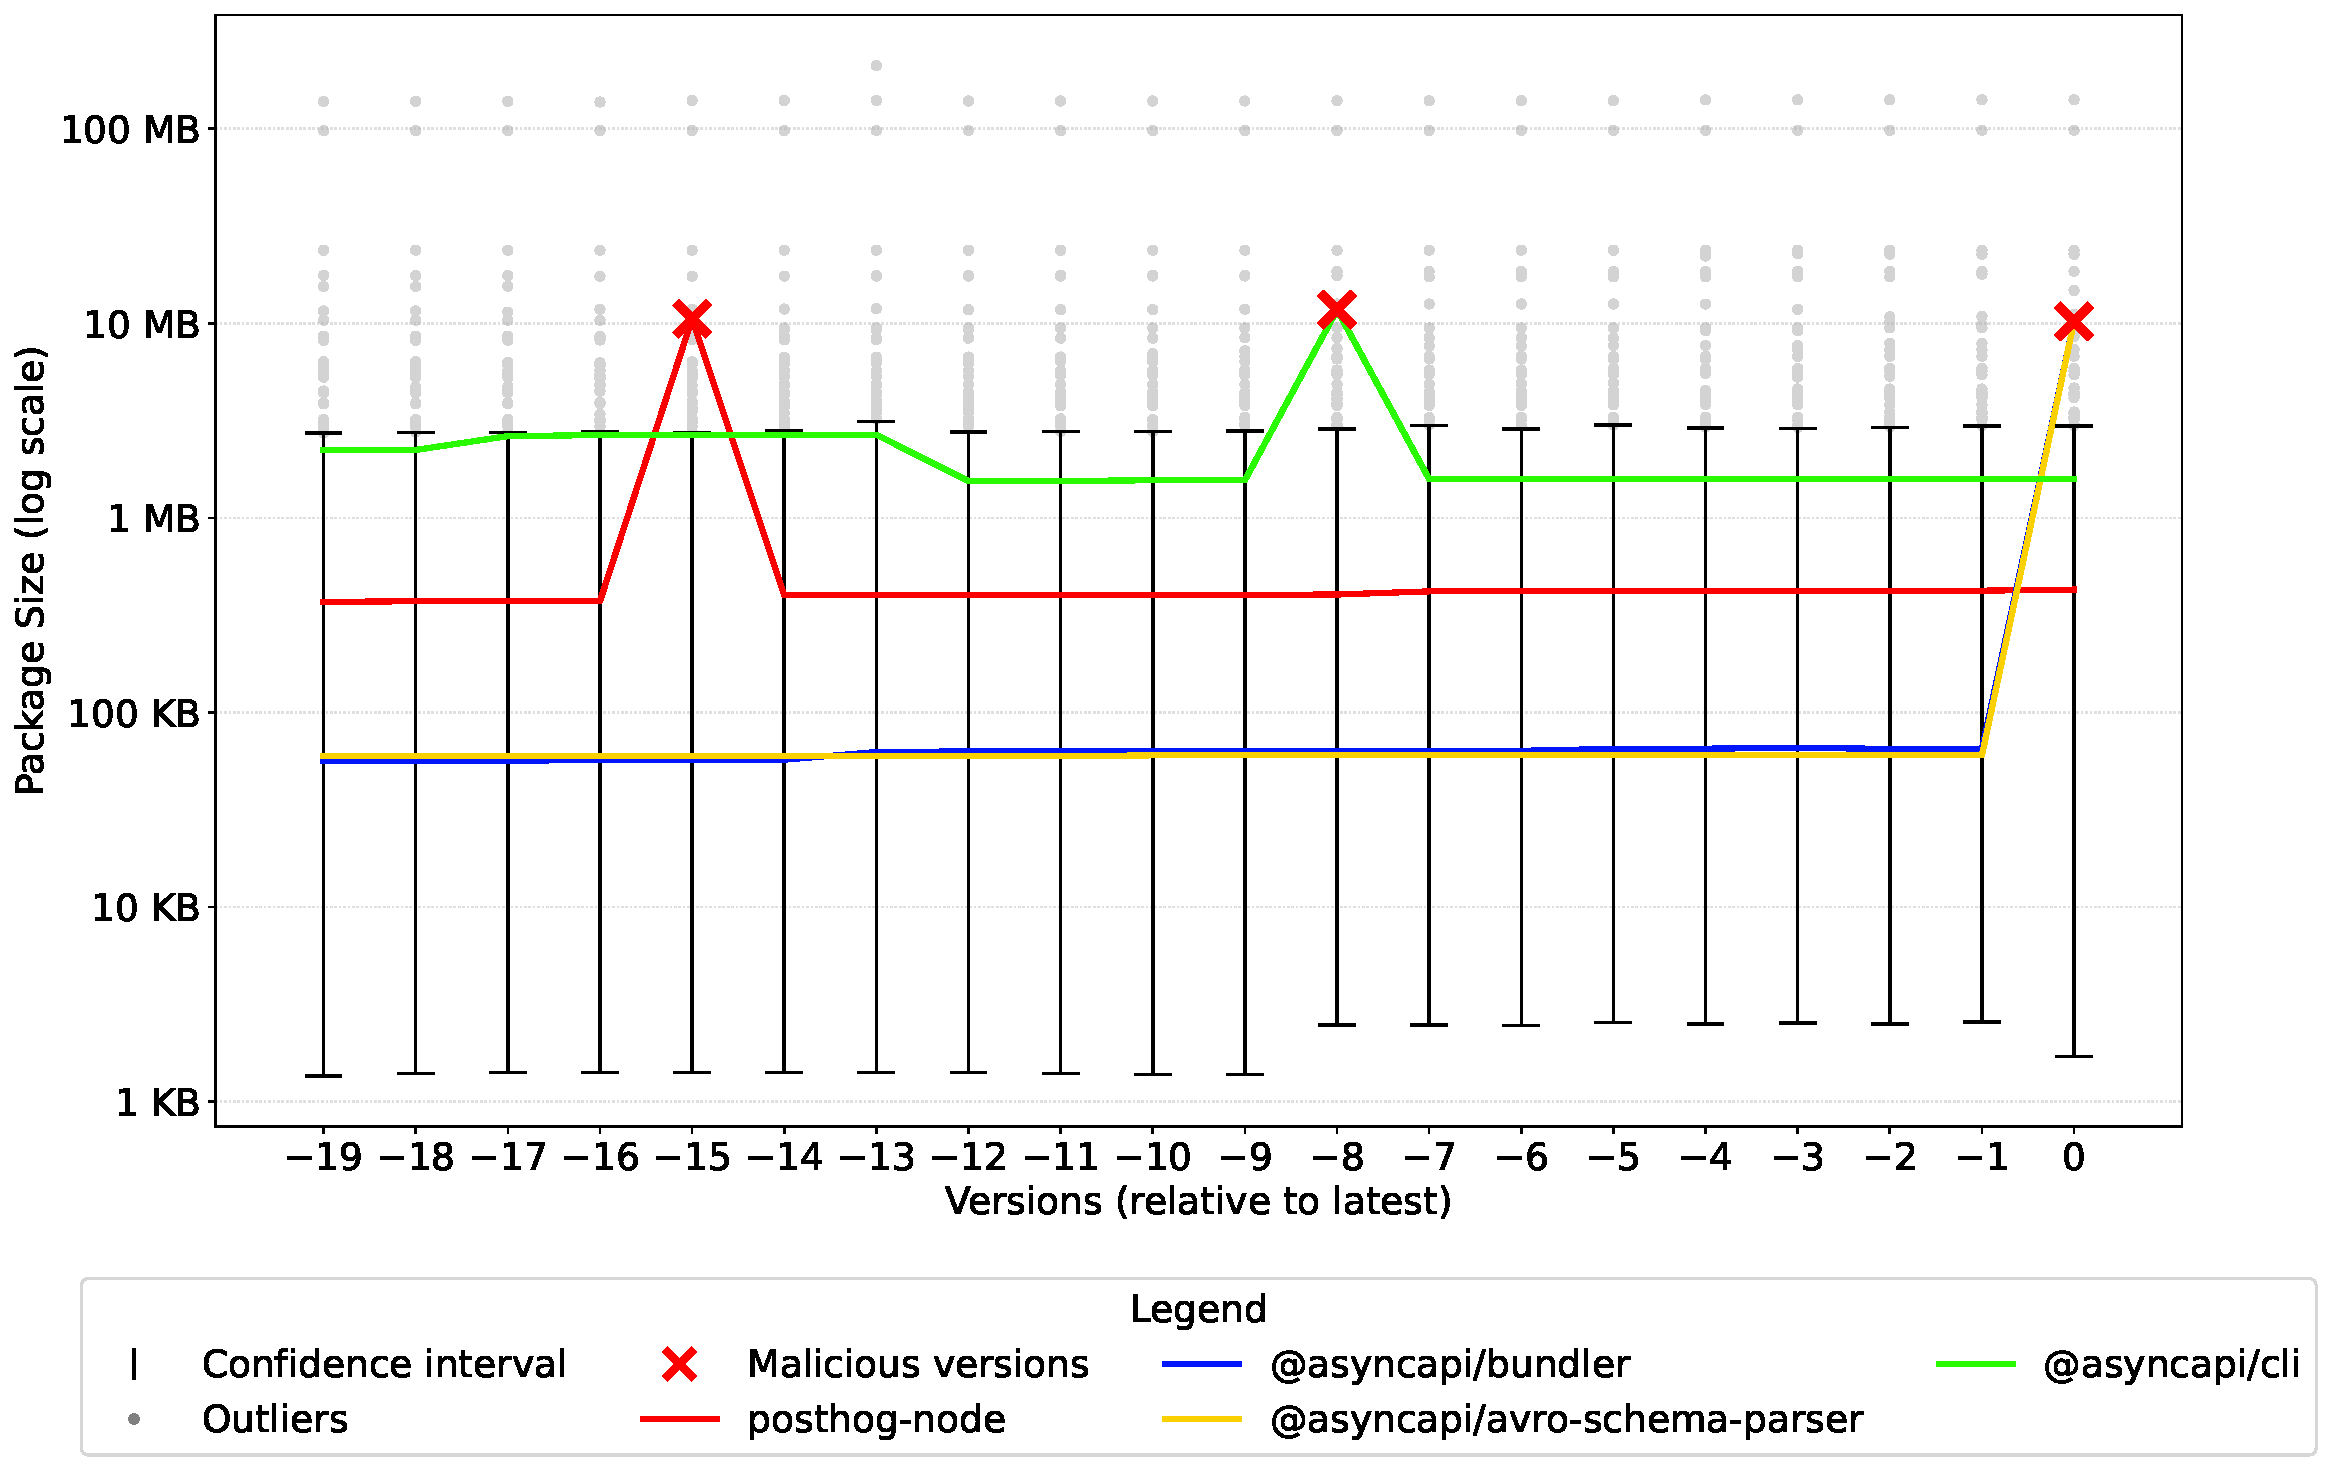
\includegraphics[width=\textwidth]{metrics/packageSize/PS_plot2single_AttackD.pdf}
    \caption{Package Size Metric: Malware Comparison for Attack D.}
    \label{fig:fig2PackageSizeAttackD}
\end{figure}

\textbf{Attack~A} (\cref{sec:attackA}) adds a malicious \ac{DLL} of 1.2~MB to each compromised package,
and as shown in \cref{fig:fig2PackageSizeAttackA}, 
this increase is insufficient to place the compromised versions among the outlier values of the Goodware dataset.
The reason is that these affected tarball are small enough to remain within the confidence intervals, 
failing to surpass the upper bound (2.7-2.9$\sim$~MB) required for outlier classification.
The metric is therefore not able to detect this specific attacks and results as not indicative.

\textbf{Attack~B} (Crypto attack, \cref{sec:attackB}) adds a single obfuscated line to an existing \texttt{index.js} file.
This increase is modest relative to the size range of the Goodware dataset, 
and as shown in \cref{fig:fig2PackageSizeAttackB}, the compromised versions remain within the confidence interval, 
making the metric not indicative for this attack.

\textbf{Attack~C} (\texttt{Shai-Hulud}~1.0, \cref{sec:attackC}) injects a new file of approximately 3.7~MB.
For the affected packages this addition is large enough to exceed the 95th percentile threshold,
placing the compromised versions among the outliers, as shown in \cref{fig:fig2PackageSizeAttackC}.
The metric is therefore effective for detecting Attack~C.

\textbf{Attack~D} (\texttt{Shai-Hulud}~2.0, \cref{sec:attackD}) introduces a file of over 10~MB.
As shown in \cref{fig:fig2PackageSizeAttackD}, this places the compromised versions well outside the outlier range,
making the metric clearly effective for detecting Attack~D.

In summary, the \emph{Package Size} metric effectively detects the two attacks that introduce large malicious files (Attacks~C and~D),
but is not sensitive enough to detect the smaller injections of Attacks~A and~B.